\chapter{Identification and Authentication}
\label{chapter:authentication}
\section{Identification}
The identity of an entity shall have the following properties:
\begin{itemize}
    \item Uniqueness
    \item Unchangable Linking
    \item Lifelong validity
    \item No Transferability
\end{itemize}

In order to identify an entity, an \emph{identifier} has to be defined. The
identifier should meet the above criteria and should be able to determine an
identity \textit{within a given context}.

Identifiers have the purpose of both accountability and access control. They can
be applied to both subjects (users, processes, ...) and objects (files, URLs,
...), humans and machines, and can be temporary or persistent.

For authentication, a separate \textit{proof of identity} is usually required:

\section{Authentication}
Authentication is the process of confirming whether a second party is indeed who
they claim to be, to a specified level of confidence. There are three basic
forms of authentication:

\begin{itemize}
    \item \emph{Something you know} (passwords)
    \item \emph{Something you have} (smart cards)
    \item \emph{Something you are} (biometrics)
\end{itemize}

Combinations of those increase the security
(\emph{Multi-Factor-Authentication}).

\paragraph{Password Authentication} is based on the \textit{something you know}
factor. Examples include unix passwords, PINs or secret code words. They can
also easily be used to authenticate groups, by distributing the password to
every entity in the group. A weakness of passwords is that an attacker can learn
and reuse it. A possible solution are \textit{one-time passwords}.

\paragraph{One-time Passwords} are only used once, an example would be a TAN
list for online banking. They can also be part of a challenge-response-protocol,
where the two parties agree on a secret function beforehand, and authentication
happens by verifying the function response to a challenge.

\paragraph{Hardware Tokens} take a similar approach in generating some kind of
one-time use token, but those are generated by dedicated hardware, shifting the
factor to \textit{something you have}. They might have an additional input such
as a pin, or, as in the case of popular 2FA solutions, the current time. The
\emph{HOTP} (HMAC-based One-Time Password algorithm) generates short time
passwords using a counter (time) and a pre-shared secret key.

\paragraph{Biometric Authentication} has to be differentiated into
\textit{verification} and \textit{recognition}. In verification, the used
specifies its identity, and the system authenticates the used if biometric
verification succeeds. In recognition, the system recognizes the user amongst
multiple known users without further input.

Biometric authentication systems can fail in two ways: \emph{False negative}
means that a user is incorrectly rejected, a \emph{false positive} means that a
user is wrongly accepted. The threshold on accepting a authentication attempt
has to be chosen in a application specific way, depending on which fault is more
acceptable. \Cref{fig:eer} shows the relationship between the \textit{False
Acceptance Rate} and \textit{False Rejection Rate} with a varying threshold. A
measure of the security of the authentication system could be the \textit{Equal
Error Rate}.
\begin{figure}
    \centering
    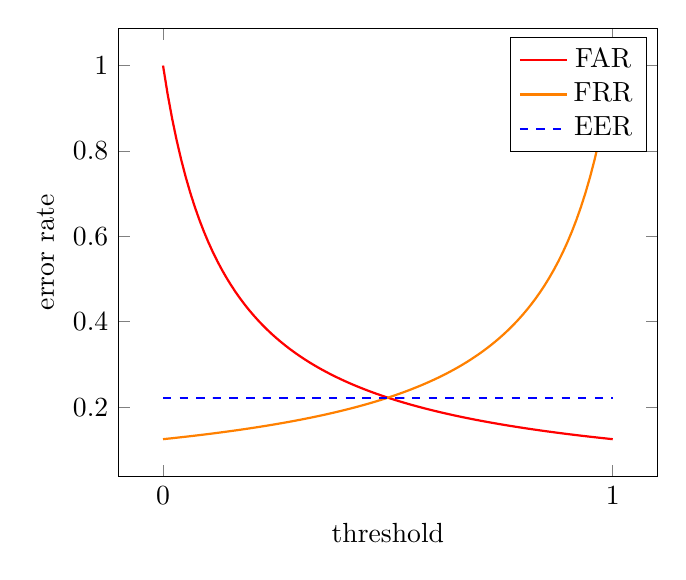
\begin{tikzpicture}
        \begin{axis}[
                xlabel=threshold,
                ylabel=error rate,
                xtick={1,8},
                xticklabels={0,1}
            ]
            \addplot[
                domain=1:8,
                samples=100,
                thick,
                color=red]{1/x};
            \addlegendentry{FAR};
    
            \addplot[
                domain=1:8,
                samples=100,
                thick,
                color=orange]{1/(9-x)};
            \addlegendentry{FRR};
    
            \addplot[
                domain=1:8,
                samples=100,
                dashed,
                thick,
                color=blue]{2/9};
            \addlegendentry{EER};
        \end{axis}
    \end{tikzpicture}
    \caption{\textit{False Acceptance Rate} and \textit{False Rejection Rate}
    for biometric authentication}
    \label{fig:eer}
\end{figure}

\section{Password Security}
Passwords which are short or badly chosen can easily be cracked. Brute-force or
dictionary attacks guess the password either randomly of from a list of known
(pass-)words. Brute-force attacks are easily feasible for passwords up to
\textasciitilde 8 characters in length, useful rules on possible guesses and
dictionary attacks can lead to success for even longer passwords. An advantage
for the attacker is when the attack can be executed \textit{offline}, such as by
stealing the file containing the password hashes. This removes the bottleneck of
the authentication mechanism of the target and allows for distributed attacks.

A common protection measure is to use a \emph{SALT}. A salt is a random value
that gets appended to the password before hashing, and then gets stored
alongside the password hash. While this does not protect a single password
against the mentioned attacks, it prevents reuse of a hash that has already been
calculated. Otherwise, it would be possible to just compare the hashes to known
hashes of popular passwords.

Another consideration is access to the password hashes. While the actual
cryptographic security is only influenced by the hash function, preventing
offline attacks by properly protecting the hashes forces the attacker to execute
much slower online attacks. Those online attacks can be slowed even further by
limiting the number of invalid authentication attempts or introducing an
increasing delay after failed authentication attempts (\textit{back off}), and
by using ``slow'' hash functions. The previously popular measure of password
aging (requiring passwords to be changed after a certain amount of time) is
discouraged, since it promotes the use of weak but easy to remember passwords.

Other attacks focus on the specific implementation of the authentication
mechanism and exploit vulnerabilities that allow login even without actually
obtaining the correct password, or allow changing or resetting passwords even
with insufficient privileges.

\subsection{Time Memory Trade-off}
In attacks on passwords a trade-off between time and memory has to be made, the
two extremes being the brute-force attack and the fully pre-calculated
dictionary/codebook attack.

One possible solution is a \emph{Variable Length Lookup Table}. Those rely on
hash chains: For many initial values, a chain of hashes (length $n_\text{max}$)
each is calculated. Only the initial and end-value are for each chain is then
stored. When a certain hash shall then be cracked, it will be hashed
$n_\text{max}$ times until a chain is found which end-state matches the
calculated hash. Once the chain is found, it can be restored using the stored
initial state which results in a chain containing the to-be-cracked hash and the
password as the state immediately preceding that value.

An improvement to lookup time can be made by making the chains variable length,
and introducing an end criterion, for example a certain number of zero-bits at
the end of the hash (\emph{Distinguished Codepoints}). This reduces the number
of end-lookups significantly.

Duplication arising from hash collisions are addressed by \emph{Rainbow Tables}:
A round-specific reduction function (hash space \textrightarrow password space)
is introduced. So even if a state is already present in a different chain (but
at another round in the chain), the original chain continues separately.

\section{Network Authentication}
The challenge of network authentication is that the communication has to be
established over an insecure channel. Passwords shall not be transmitted as
plaintext, but in encrypted form. Thus the problem quickly changes from
authentication to a key-distribution problem.

\subsection{Kerberos}
Kerberos is a network authentication protocol using symmetric cryptography. It
is best explained using an example:

Each organization has one authentication server, also called key distribution
center, and a ticket granting server TGS. The TGS hands out the authorization to
clients to use a certain service. This is done using tickets. A ticket for a
client to access a service includes a specific session key, the identity of the
client and a validity period. The ticket is encrypted using a key that only the
TGS and the service know. The client can not decrypt the ticket.

If a client $A$ wants to access a service $B$, $A$ first contacts the
authentication server. The server then provides $A$ with a session key between
$A$ and the TGS (encrypted using $A$s password), and a ticket for the TGS which
can provide TGS with the session key to talk to $A$.

The TGS can now provide $A$ with a session key between $A$ and $B$, and a ticket
for $B$ that provides $B$ with the session key.

Now $A$ and $B$ have a shared session key, and they can communicate.

Criticism of kerberos include the centrally controlled servers, and reliance on
synchronized clocks for timestamps. Session keys are known to the servers, not
only to the client and service. Also, the first message is not authenticated,
opening multiple attack vectors.

\subsection{Station to Station}
It has already been established that Diffie-Hellman is susceptible to
man-in-the-middle attacks (\cref{sec:diffiehellman}). A solution is to
authenticate the public keys $A$ and $B$ using digital signatures.

The station to station protocol now requires verification of signatures after
exchanging the public values $A$ and $B$: Bob signs both $A$ and $B$ with his
private signing key, Alice signs both $A$ and $B$ using her private signing key.
The signatures are encrypted using the shared secret key. Verification of the
signature now assures each party that no man in the middle who is exchanging the
keys is present.

This assumes however that the public signature verification keys are already
known.

\subsection{Perfect Forward Secrecy}
Perfect forward secrecy is given when the compromise of a long term secret such
as secret keys does not compromise the security of short term secrets used in
the past.

\subsection{Certificates}
A digital certificate links some public key to a person. The certificates
generally includes the public key, some identifier and a validity period. All
this is signed by the signature generation key of a trusted third party
(certification authority CA). This certificate can then be verified if the
verification key of the CA is known.

The \emph{certification authorities} play an important role in the \emph{public
key infrastructure}. Usually a number of CAs exist, which all operate under some
root CA. The root CA signs the public keys of the other CAs and such verifies
the validity of the CA. Those CAs can then sign public keys of users, after
verifying their identity.

The public key of the root CA has to be transmitted using a secure channel. This
is usually done by distribution via operating systems and browsers.

\subsubsection{X.509 Certificates}
X.509 is a standard for digital certificates. It specifies that the identifier
is in the hierarchical \textit{distinguished name (DN)} naming format. It also
specifies the fields in the certificate:
\begin{itemize}
    \item Version
    \item Serial number
    \item Signature algorithm
    \item Issuers DN
    \item Validity interval
    \item Subjects DN
    \item Subjects public key
    \item Issuers unique identifier
    \item Subjects unique identifier
    \item Extensions
    \item Signature
\end{itemize}
Extensions can for example control the key usage (signing emails, TLS web
server, etc).

PKIs have several problems, which become evident if a CA gets compromised. This
allows the attacker to for example issue certificates for any domain. The number
of CAs commonly in use is large, and many use weak security.

\subsection{PGP}
Pretty Good Privacy PGP provides an alternative approach to trust in a
decentralized fashion. It relies on the concept of users singing each others
keys. Each user has a keyring of public keys and signatures on them. If a user
receives a public key which is signed by many users they trust, they might also
trust the new public key.

There are different notions of trust: \emph{Owner trust} is the value of trust
someone assigns to a key in the keyring. Completely trusting a key implies also
trusting the other keys signed by this key.

\emph{Calculated trust} answers the question of whether to trust a public key
that was used. A chain of signatures is required, starting with some public key
in the keyring and ending with the key in question.

\emph{Key legitimacy} is calculated as
\begin{equation}
    L = \frac{x}{X}+\frac{y}{Y}
\end{equation}
with $x$ being the number of signatures with ``marginal'' trust, $y$ the number
of signatures with ``complete'' trust and $X$ and $Y$ the required corresponding
number of signatures.
